\documentclass{article}

\usepackage[utf8]{inputenc}
\usepackage[portuguese]{babel}
\usepackage{blindtext}
\usepackage{graphicx}
\usepackage{amsmath}
\usepackage{float}
\usepackage{caption}
\usepackage[compact]{titlesec}
\usepackage{multicol}
\usepackage[a4paper, total={7.5in, 10in}]{geometry}
\usepackage[font=scriptsize,labelfont=bf]{caption}
\usepackage{listings}
\usepackage{color}
 
\definecolor{codegreen}{rgb}{0,0.6,0}
\definecolor{codegray}{rgb}{0.5,0.5,0.5}
\definecolor{codepurple}{rgb}{0.58,0,0.82}
\definecolor{backcolour}{rgb}{0.95,0.95,0.92}
 
\lstdefinestyle{mystyle}{
    backgroundcolor=\color{backcolour},   
    commentstyle=\color{codegreen},
    keywordstyle=\color{magenta},
    numberstyle=\tiny\color{codegray},
    stringstyle=\color{codepurple},
    basicstyle=\footnotesize,
    breakatwhitespace=false,         
    breaklines=true,                 
    captionpos=b,                    
    keepspaces=true,                 
    numbers=left,                    
    numbersep=5pt,                  
    showspaces=false,                
    showstringspaces=false,
    showtabs=false,                  
    tabsize=2
}
 
\lstset{style=mystyle}

\setlength{\columnsep}{1cm}
\setlength{\parindent}{0em}
\titlespacing{\section}{1pt}{*0.5}{*0.5}
\begin{document}

\textbf{Relatório de Entrega de Trabalho} \newline
\textbf{Disciplina de Programação Paralela (PP)}\textbf{ - Prof. César De Rose} \newline
\textbf{Alunos:} Rafael Rios e Rodrigo Silveira \newline
\textbf{Exercício:} TPP1: MPI Mestre/Escravo (ME) \newline

\begin{multicols*}{2}

\section{Implementação}
O objetivo deste trabalho foi compreender e avaliar o desempenho do mestre/escravo, um dos modelos básicos de aplicações paralelas. Para isto, implementou-se um código que distribui a carga de trabalho entre diversos processos (escravos), controlados somente pelo processo raiz (ID = 0). Os algoritmos utilizados para os testes foram o quicksort e o bubblesort. No primeiro caso, a carga foi de 1.000 vetores contendo 100.000 valores para serem ordenados; no segundo, devido ao menor desempenho do bubblesort, foram utilizados 1.000 vetores contendo apenas 10.000 valores. Cada escravo recebe um vetor por vez e, uma vez processado, o envia para o mestre e aguarda uma mensagem sinalizando que um novo vetor deve ser processado (WORKTAG) ou uma mensagem de suicídio (KILLTAG). \newline
A maior parte da implementação está na parte do mestre, uma vez que ele é responsável pelo controle da divisão da carga de trabalho entre os escravos. Sendo assim, o código dos escravos se resume basicamente a um laço infinito em que se aguarda uma mensagem do mestre, se a mensagem conter a tag 'KILLTAG', o escravo deve escapar do laço e terminar a execução, senão ele aplica o algoritmo de ordenamento escolhido (quicksort ou bubblesort) ao vetor e envia o vetor, agora ordenado, para o mestre. O código do mestre utiliza o vetor controle como uma maneira de organizar qual vetor cada escravo está executando. O vetor controle possui o tamanho igual ao número de escravos, e, desse modo, associa-se a ID de cada escravo a um índice do vetor. Por exemplo, se o escravo 2 estiver processando o vetor 592, a posição (2-1) do vetor controle recebe o valor 592, quando o mestre receber a resposta desse escravo, sinaliza-se que o escravo está sem processar colocando o valor 0 à posição (2-1) do vetor controle. A lógica do mestre divide-se em três partes, inicialmente, é enviado a cada um dos escravos um vetor do saco, uma vez que sabe-se que no início da execução todos os escravos estão aguardando trabalho. A seguir, enquanto o último vetor que foi enviado não for o último vetor do saco, se verifica se algum escravo retornou um vetor utilizando MPI\_Probe, quando esta função retorna, a ID do processo que terminou de processar o vetor é guardada na variável status.MPI\_SOURCE. Em seguida, utiliza-se o vetor de controle para saber qual era a posição dentro do saco do vetor que foi processado e chama-se a função MPI\_Recv para receber o vetor e atualizar o saco. Agora que um escravo está aguardando processamento, atribui-se um novo vetor do saco a este escravo através do vetor controle e a carga é mais uma vez enviada através da função MPI\_Send. A terceira parte da lógica do escravo consiste em percorrer o vetor de controle e verificar se o valor de cada posição é 0. Caso for 0, envia-se ao escravo correspondente a mensagem de suicídio, caso for um valor diferente de 0, significa que o escravo correspondente ainda está processando algum vetor, nesse caso, o mestre aguarda a resposta do escravo e logo em seguida envia a mensagem de suicídio.

\section{Dificuldades encontradas}
Inicialmente, obteve-se certa dificuldade em verificar se o algoritmo de quicksort estava sendo executado corretamente e se todos os vetores do saco eram processados, devido às complicações que se encontram ao tentar depurar códigos concorrentes. Depois, o problema foi de performance, uma vez que o código sequencial executava muito mais rapidamente que a versão paralela quando distribuída em mais de uma máquina. Este problema foi solucionado ao alocar nodos com exclusividade na máquina grad, em vez de compartilhados.

\section{Testes}
Foram realizados testes com alocação de 2 nodos na grad, executando o código do mestre escravo paralelo para 4 até 32 processos, aumentando o número de 4 em 4, totalizando 8 execuções para cada um dos ordenamentos. O código sequencial foi executado em um computador pessoal com um processador Intel I5-7400 (4 núcleos e 4 threads - 3.0GHz) e 16GB de memória RAM, obtendo 189,238s para o bubblesort e 4,918s para o quicksort.

\section{Análise de desempenho}
As versões paralelas tanto do quicksort quanto do bubblesort obtiveram um desempenho muito superior às sequenciais dos respectivos algoritmos. Nos testes executados, percebeu-se que para um número maior que aproximadamente 16 processos, não obteve-se ganhos de performance significativos, e com a inclusão de mais processos, a eficiência por processo reduziu-se cada vez mais, isso se deve ao overhead de comunicação gerado pela troca de mensagens e também pelo fato de que todos os escravos são gerenciados por um único mestre, que acaba se tornando o gargalo da aplicação.

\section{Observações Finais}
A utilização do modelo mestre/escravo se mostrou eficiente para os algoritmos tanto do quicksort quanto do bubblesort com a carga de 1.000 vetores de 100.000 valores no caso do quicksort e de 1.000 vetores de 10.000 valores no caso do bubblesort. Obteve-se um speedup significativo ao se comparar as versões paralelas às sequenciais. Também foi possível perceber a degradação do desempenho ao ultrapassar um certo número de processos, devido ao overhead da troca de mensagens e pelo gargalo ocasionado pelo fato de todo processamento ter que ser gerenciado pelo único processo mestre. Não obstante, para um número tanto pequeno quanto elevado de processos, os tempos de execução dos códidos paralelos foram consideravelmente menores que os tempo dos códigos sequenciais.

\end{multicols*}

\newpage

\begin{figure}[H]
            \centering
            \vspace{-0.3em}
            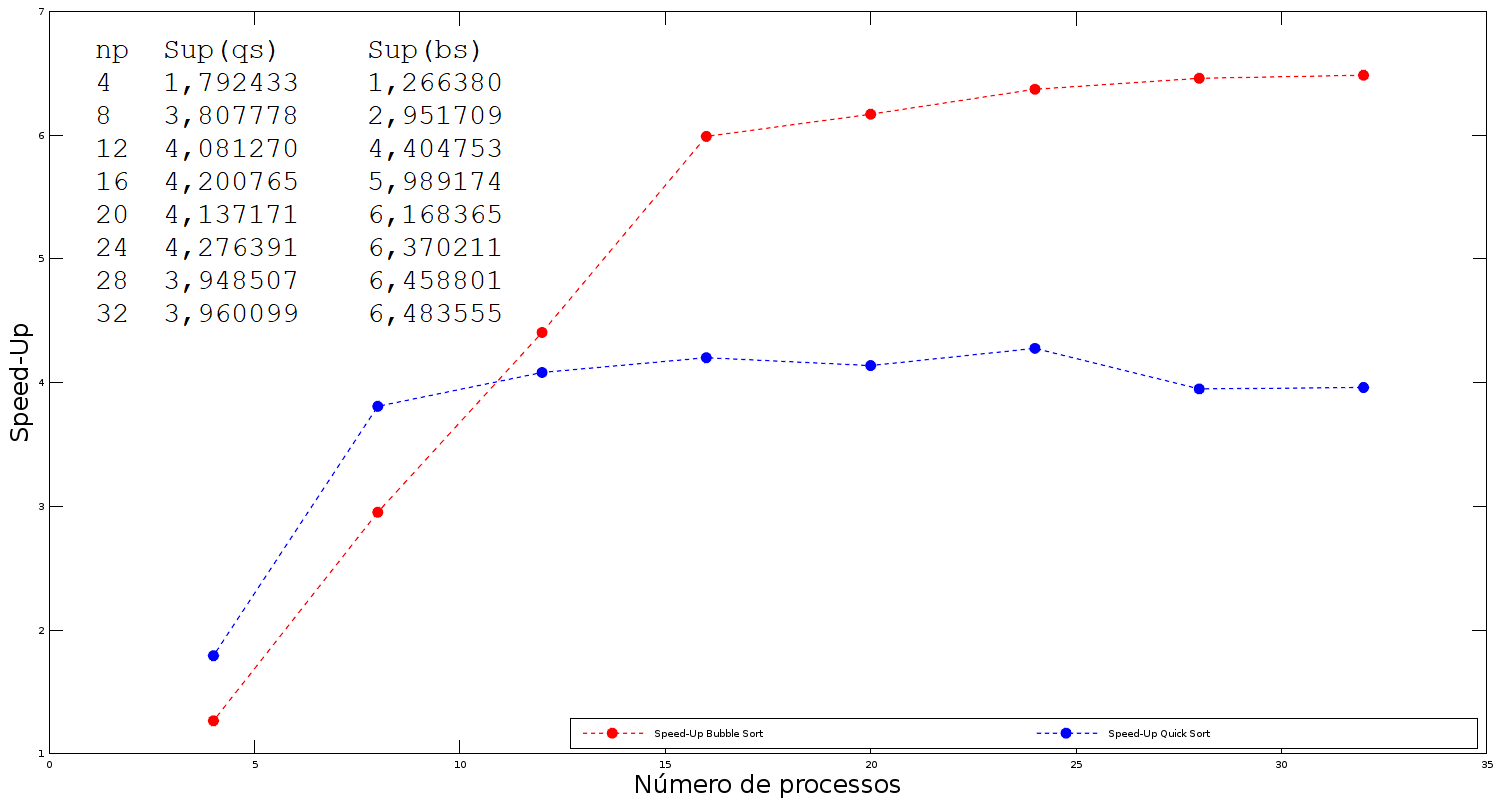
\includegraphics[width=14cm, height=7cm]{speedup_vals.png}
            \vspace{-0.6em}
            \caption{Gráfico com Speed-Up para Quick sort e Bubble sort}
            \vspace{-1.1em}
\end{figure}

\begin{figure}[H]
            \centering
            \vspace{-0.3em}
            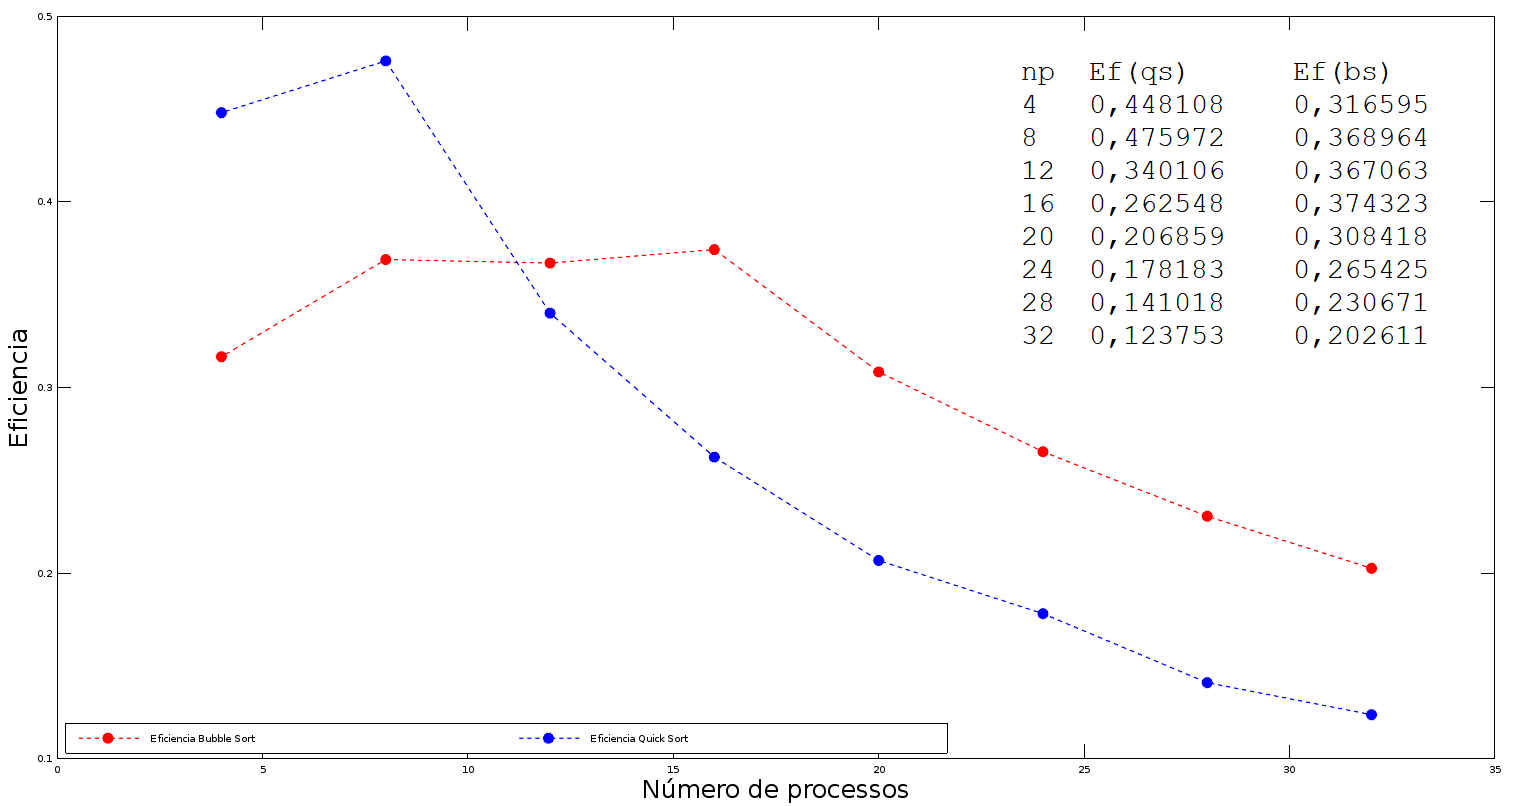
\includegraphics[width=14cm, height=7cm]{eficiencia_vals.png}
            \vspace{-0.6em}
            \caption{Gráfico com Eficiência para Quick sort e Bubble sort}
            \vspace{-1.1em}
\end{figure}

\newpage

\lstinputlisting[language=C++]{master_slave.c}

\newpage

\lstinputlisting[language=C++]{ms_sequencial.c}
\end{document}
